\chapter{Introduction \`a l'Apprentissage Automatique}
\label{ch:ml_intro}

\section{Qu'est-ce que l'apprentissage automatique~?}

\begin{definition}[Apprentissage automatique]
L'\textbf{apprentissage automatique}\index{apprentissage automatique} (\textit{machine learning}, ML) est une branche de l'intelligence artificielle qui permet aux ordinateurs d'apprendre \`a partir de donn\'ees sans \^etre explicitement programm\'es pour chaque t\^ache.
\end{definition}

\begin{intuition}
Plut\^ot que d'\'ecrire des r\`egles manuellement (par exemple, <<~si le client a plus de 30 ans et un revenu sup\'erieur \`a 50\,000\,€, alors approuver le pr\^et ~>>), on fournit des \textbf{exemples} au mod\`ele qui d\'ecouvre lui-m\^eme les r\`egles sous-jacentes.
\end{intuition}

\subsection{Types d'apprentissage}

\index{apprentissage supervis\'e}\index{apprentissage non supervis\'e}\index{apprentissage par renforcement}

\begin{center}
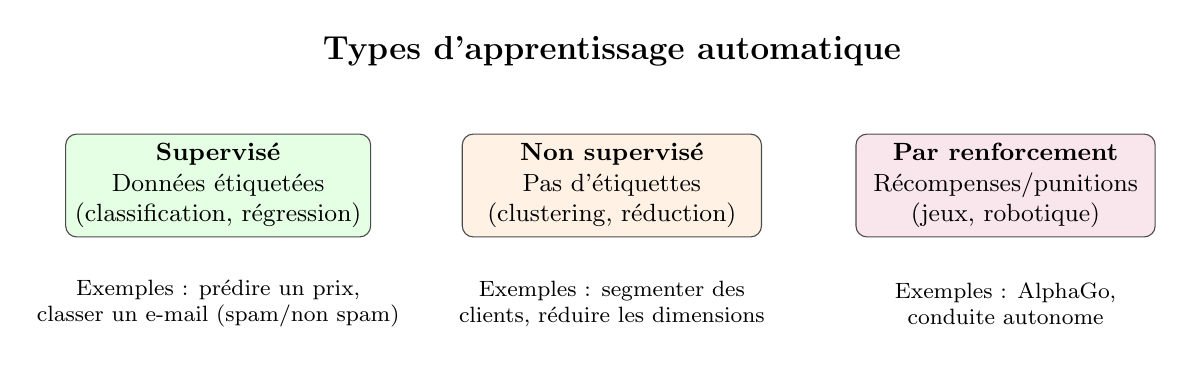
\begin{tikzpicture}[
    box/.style={rectangle, draw=black!70, fill=blue!8, rounded corners, minimum width=3.8cm, minimum height=1.2cm, align=center, font=\small},
    title/.style={font=\bfseries\large}
]
\node[title] at (0, 3.2) {Types d'apprentissage automatique};
\node[align=center,box, fill=green!10] (sup) at (-5, 1.5) {\textbf{Supervis\'e}\\Donn\'ees \'etiquet\'ees\\(classification, r\'egression)};
\node[align=center,box, fill=orange!10] (unsup) at (0, 1.5) {\textbf{Non supervis\'e}\\Pas d'\'etiquettes\\(clustering, r\'eduction)};
\node[align=center,box, fill=purple!10] (reinf) at (5, 1.5) {\textbf{Par renforcement}\\R\'ecompenses/punitions\\(jeux, robotique)};

\node[font=\footnotesize, align=center] at (-5, 0) {Exemples~: pr\'edire un prix,\\classer un e-mail (spam/non spam)};
\node[font=\footnotesize, align=center] at (0, 0) {Exemples~: segmenter des\\clients, r\'eduire les dimensions};
\node[font=\footnotesize, align=center] at (5, 0) {Exemples~: AlphaGo,\\conduite autonome};
\end{tikzpicture}
\end{center}

\begin{definition}[Apprentissage supervis\'e]
On dispose de paires $(\mathbf{x}_i, y_i)$ o\`u $\mathbf{x}_i$ sont les \textbf{variables explicatives}\index{variables explicatives} (\textit{features}) et $y_i$ est la \textbf{cible}\index{cible} (\textit{target}). Le mod\`ele apprend une fonction $f$ telle que $f(\mathbf{x}_i) \approx y_i$.
\begin{itemize}
    \item \textbf{Classification}\index{classification}~: $y$ est une cat\'egorie (spam/non spam, esp\`ece de fleur).
    \item \textbf{R\'egression}\index{r\'egression}~: $y$ est une valeur continue (prix, temp\'erature).
\end{itemize}
\end{definition}

\begin{definition}[Apprentissage non supervis\'e]
On dispose uniquement de $\mathbf{x}_i$ sans \'etiquettes. Le mod\`ele cherche des \textbf{structures cach\'ees} dans les donn\'ees (groupes, axes principaux).
\end{definition}

\section{Le flux de travail en apprentissage supervis\'e}
\label{sec:workflow_ml}

\index{train/test split}\index{d\'ecoupage entra\^inement/test}

\begin{center}
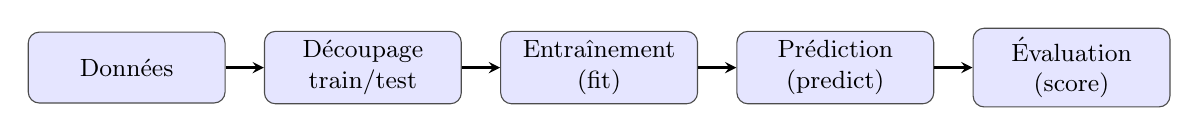
\begin{tikzpicture}[
    stepbox/.style={rectangle, draw=black!70, fill=blue!10, rounded corners, minimum width=2.5cm, minimum height=0.9cm, align=center, font=\small},
    arr/.style={->, thick, >=stealth}
]
\node[stepbox] (data) at (0,0) {Donn\'ees};
\node[align=center,stepbox] (split) at (3,0) {D\'ecoupage\\train/test};
\node[align=center,stepbox] (train) at (6,0) {Entra\^inement\\(\py{fit})};
\node[align=center,stepbox] (pred) at (9,0) {Pr\'ediction\\(\py{predict})};
\node[align=center,stepbox] (eval) at (12,0) {\'Evaluation\\(\py{score})};

\draw[arr] (data) -- (split);
\draw[arr] (split) -- (train);
\draw[arr] (train) -- (pred);
\draw[arr] (pred) -- (eval);
\end{tikzpicture}
\end{center}

\begin{enumerate}
    \item \textbf{Collecte et pr\'eparation} des donn\'ees.
    \item \textbf{D\'ecoupage} en ensemble d'entra\^inement\index{ensemble d'entra\^inement} et ensemble de test\index{ensemble de test}.
    \item \textbf{Entra\^inement} du mod\`ele sur les donn\'ees d'entra\^inement.
    \item \textbf{Pr\'ediction} sur les donn\'ees de test.
    \item \textbf{\'Evaluation} des performances.
\end{enumerate}

\begin{codeblock}[title=\textbf{Python}]
\begin{minted}{python}
from sklearn.model_selection import train_test_split
from sklearn.datasets import load_iris

# Chargement des donn\'ees
iris = load_iris()
X, y = iris.data, iris.target

# D\'ecoupage : 70% entra\^inement, 30% test
X_train, X_test, y_train, y_test = train_test_split(
    X, y, test_size=0.3, random_state=42
)
print(f"Entra\^inement : {X_train.shape[0]} \'echantillons")
print(f"Test : {X_test.shape[0]} \'echantillons")
\end{minted}
\end{codeblock}

\begin{codeoutput}
\begin{minted}{text}
Entra\^inement : 105 \'echantillons
Test : 45 \'echantillons
\end{minted}
\end{codeoutput}

\section{L'API Scikit-learn}
\label{sec:api_sklearn}

\index{scikit-learn}\index{fit}\index{predict}\index{score}

\begin{bonnepratique}
Tous les mod\`eles scikit-learn suivent la m\^eme interface~:
\begin{enumerate}
    \item \py{modele = Classe(param\`etres)} --- cr\'eer le mod\`ele.
    \item \py{modele.fit(X_train, y_train)} --- entra\^iner.
    \item \py{modele.predict(X_test)} --- pr\'edire.
    \item \py{modele.score(X_test, y_test)} --- \'evaluer.
\end{enumerate}
\end{bonnepratique}

\subsection{Exemple complet~: k plus proches voisins sur Iris}

\index{k plus proches voisins}\index{KNN}

\begin{codeblock}[title=\textbf{Python}]
\begin{minted}{python}
from sklearn.neighbors import KNeighborsClassifier
from sklearn.metrics import accuracy_score

# Cr\'eation du mod\`ele KNN avec k=5
knn = KNeighborsClassifier(n_neighbors=5)

# Entra\^inement
knn.fit(X_train, y_train)

# Pr\'ediction
y_pred = knn.predict(X_test)

# \'Evaluation
acc = accuracy_score(y_test, y_pred)
print(f"Pr\'edictions : {y_pred[:10]}")
print(f"V\'erit\'e     : {y_test[:10]}")
print(f"Exactitude  : {acc:.4f}")
\end{minted}
\end{codeblock}

\begin{codeoutput}
\begin{minted}{text}
Pr\'edictions : [1 0 2 1 1 0 1 2 1 1]
V\'erit\'e     : [1 0 2 1 1 0 1 2 1 1]
Exactitude  : 1.0000
\end{minted}
\end{codeoutput}

\begin{remarque}
La m\'ethode \py{score()} renvoie l'\textbf{exactitude}\index{exactitude} (\textit{accuracy}) pour la classification et le \textbf{coefficient de d\'etermination} $R^2$ pour la r\'egression.
\end{remarque}

\section{Sur-apprentissage et sous-apprentissage}
\label{sec:overfitting}

\index{sur-apprentissage}\index{sous-apprentissage}\index{biais}\index{variance}

\begin{definition}[Sur-apprentissage et sous-apprentissage]
\begin{itemize}
    \item \textbf{Sous-apprentissage}\index{sous-apprentissage} (\textit{underfitting})~: le mod\`ele est trop simple, il ne capture pas la structure des donn\'ees. \textbf{Biais \'elev\'e}.
    \item \textbf{Sur-apprentissage}\index{sur-apprentissage} (\textit{overfitting})~: le mod\`ele est trop complexe, il m\'emorise le bruit des donn\'ees d'entra\^inement. \textbf{Variance \'elev\'ee}.
\end{itemize}
\end{definition}

\begin{center}
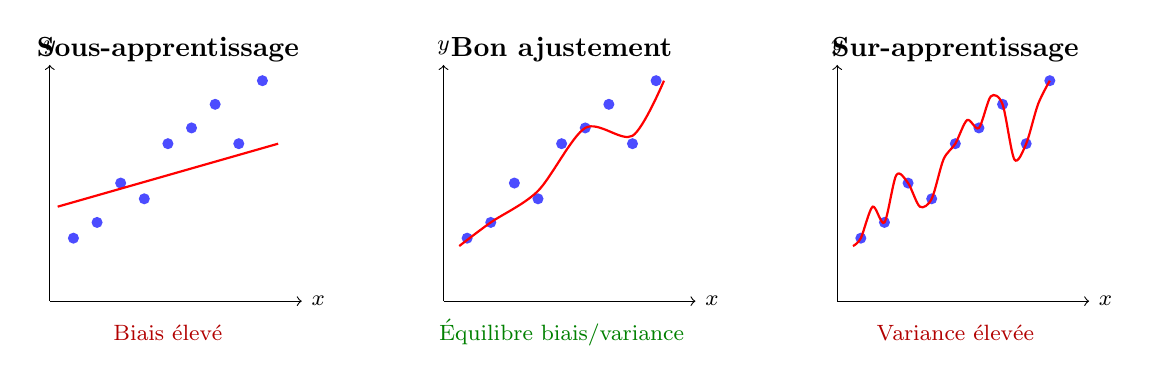
\begin{tikzpicture}
    % Sous-apprentissage
    \begin{scope}[shift={(-5,0)}]
        \node[font=\bfseries] at (1.5, 3.2) {Sous-apprentissage};
        \draw[->] (0,0) -- (3.2,0) node[right] {\footnotesize $x$};
        \draw[->] (0,0) -- (0,3) node[above] {\footnotesize $y$};
        \foreach \x/\y in {0.3/0.8, 0.6/1.0, 0.9/1.5, 1.2/1.3, 1.5/2.0, 1.8/2.2, 2.1/2.5, 2.4/2.0, 2.7/2.8} {
            \fill[blue!70] (\x, \y) circle (2pt);
        }
        \draw[red, thick] (0.1, 1.2) -- (2.9, 2.0);
        \node[font=\footnotesize, text=red!70!black] at (1.5, -0.4) {Biais \'elev\'e};
    \end{scope}
    % Bon ajustement
    \begin{scope}[shift={(0,0)}]
        \node[font=\bfseries] at (1.5, 3.2) {Bon ajustement};
        \draw[->] (0,0) -- (3.2,0) node[right] {\footnotesize $x$};
        \draw[->] (0,0) -- (0,3) node[above] {\footnotesize $y$};
        \foreach \x/\y in {0.3/0.8, 0.6/1.0, 0.9/1.5, 1.2/1.3, 1.5/2.0, 1.8/2.2, 2.1/2.5, 2.4/2.0, 2.7/2.8} {
            \fill[blue!70] (\x, \y) circle (2pt);
        }
        \draw[red, thick, smooth] plot coordinates {(0.2, 0.7) (0.6, 1.0) (1.2, 1.4) (1.8, 2.2) (2.4, 2.1) (2.8, 2.8)};
        \node[font=\footnotesize, text=green!50!black] at (1.5, -0.4) {\'Equilibre biais/variance};
    \end{scope}
    % Sur-apprentissage
    \begin{scope}[shift={(5,0)}]
        \node[font=\bfseries] at (1.5, 3.2) {Sur-apprentissage};
        \draw[->] (0,0) -- (3.2,0) node[right] {\footnotesize $x$};
        \draw[->] (0,0) -- (0,3) node[above] {\footnotesize $y$};
        \foreach \x/\y in {0.3/0.8, 0.6/1.0, 0.9/1.5, 1.2/1.3, 1.5/2.0, 1.8/2.2, 2.1/2.5, 2.4/2.0, 2.7/2.8} {
            \fill[blue!70] (\x, \y) circle (2pt);
        }
        \draw[red, thick, smooth] plot coordinates {(0.2, 0.7) (0.3, 0.8) (0.45, 1.2) (0.6, 1.0) (0.75, 1.6) (0.9, 1.5) (1.05, 1.2) (1.2, 1.3) (1.35, 1.8) (1.5, 2.0) (1.65, 2.3) (1.8, 2.2) (1.95, 2.6) (2.1, 2.5) (2.25, 1.8) (2.4, 2.0) (2.55, 2.5) (2.7, 2.8)};
        \node[font=\footnotesize, text=red!70!black] at (1.5, -0.4) {Variance \'elev\'ee};
    \end{scope}
\end{tikzpicture}
\end{center}

\begin{theoreme}[Compromis biais-variance]
L'erreur de g\'en\'eralisation\index{erreur de g\'en\'eralisation} d'un mod\`ele se d\'ecompose en~:
\[
\text{Erreur totale} = \text{Biais}^2 + \text{Variance} + \text{Bruit irr\'eductible}
\]
Le but est de trouver le mod\`ele qui minimise cette erreur totale, en \'equilibrant biais et variance.
\end{theoreme}

\begin{center}
\begin{tikzpicture}
    \draw[->] (0,0) -- (8,0) node[right] {Complexit\'e du mod\`ele};
    \draw[->] (0,0) -- (0,5) node[above] {Erreur};
    \draw[blue, thick, domain=0.5:7.5, smooth] plot (\x, {3.5/\x + 0.3});
    \node[blue, font=\footnotesize] at (2.5, 2.5) {Biais$^2$};
    \draw[red, thick, domain=0.5:7.5, smooth] plot (\x, {0.05*\x*\x + 0.2});
    \node[red, font=\footnotesize] at (6, 2.5) {Variance};
    \draw[black!60, thick, dashed, domain=0.5:7.5, smooth] plot (\x, {3.5/\x + 0.05*\x*\x + 0.5});
    \node[black!60, font=\footnotesize] at (5.5, 4.5) {Erreur totale};
    \draw[green!50!black, thick, dashed] (2.8, 0) -- (2.8, 4.5);
    \node[green!50!black, font=\footnotesize, align=center] at (2.8, 4.8) {Optimum};
\end{tikzpicture}
\end{center}

\section{Validation crois\'ee}
\label{sec:cross_validation}

\index{validation crois\'ee}\index{k-fold}

\begin{definition}[Validation crois\'ee \`a $k$ plis]
La \textbf{validation crois\'ee} (\textit{$k$-fold cross-validation}) divise les donn\'ees en $k$ sous-ensembles (\textit{folds}). On entra\^ine le mod\`ele $k$ fois, chaque fois en utilisant un pli diff\'erent comme ensemble de test et les $k-1$ autres comme ensemble d'entra\^inement.
\end{definition}

\begin{center}
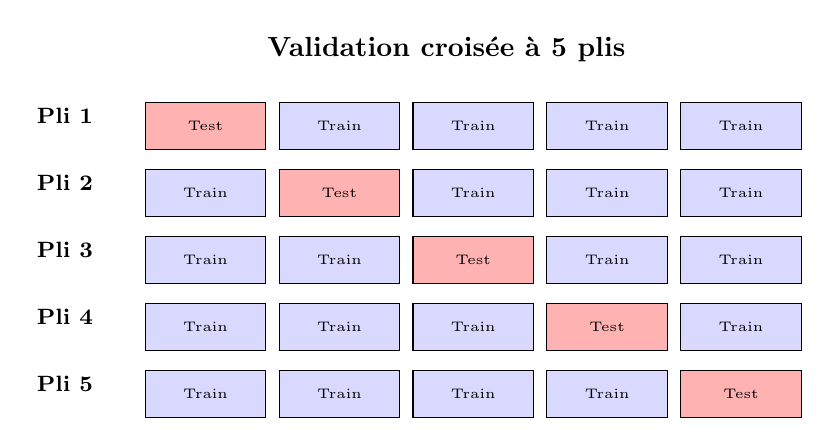
\begin{tikzpicture}[scale=0.85]
    \foreach \fold in {1,...,5} {
        \pgfmathtruncatemacro{\ypos}{-\fold}
        \node[font=\footnotesize\bfseries] at (-1.2, \ypos+0.5) {Pli \fold};
        \foreach \block in {1,...,5} {
            \pgfmathtruncatemacro{\xpos}{(\block-1)*2}
            \ifnum\block=\fold
                \fill[red!30] (\xpos, \ypos) rectangle (\xpos+1.8, \ypos+0.7);
                \draw (\xpos, \ypos) rectangle (\xpos+1.8, \ypos+0.7);
                \node[font=\tiny] at (\xpos+0.9, \ypos+0.35) {Test};
            \else
                \fill[blue!15] (\xpos, \ypos) rectangle (\xpos+1.8, \ypos+0.7);
                \draw (\xpos, \ypos) rectangle (\xpos+1.8, \ypos+0.7);
                \node[font=\tiny] at (\xpos+0.9, \ypos+0.35) {Train};
            \fi
        }
    }
    \node[font=\bfseries] at (4.5, 0.5) {Validation crois\'ee \`a 5 plis};
\end{tikzpicture}
\end{center}

\begin{codeblock}[title=\textbf{Python}]
\begin{minted}{python}
from sklearn.model_selection import cross_val_score

knn = KNeighborsClassifier(n_neighbors=5)

# Validation crois\'ee \`a 5 plis
scores = cross_val_score(knn, X, y, cv=5, scoring='accuracy')

print(f"Scores par pli : {scores}")
print(f"Moyenne : {scores.mean():.4f}")
print(f"\'Ecart-type : {scores.std():.4f}")
\end{minted}
\end{codeblock}

\begin{codeoutput}
\begin{minted}{text}
Scores par pli : [0.9667 0.9667 0.9333 0.9667 1.0000]
Moyenne : 0.9667
\'Ecart-type : 0.0211
\end{minted}
\end{codeoutput}

\begin{attention}
Ne jamais \'evaluer un mod\`ele sur les donn\'ees d'entra\^inement~! Un score parfait sur l'entra\^inement peut cacher un \textbf{sur-apprentissage} s\'ev\`ere. Utilisez toujours un ensemble de test s\'epar\'e ou la validation crois\'ee.
\end{attention}

\subsection{Choix de $k$ dans KNN}

\begin{codeblock}[title=\textbf{Python}]
\begin{minted}{python}
import numpy as np

k_values = range(1, 21)
mean_scores = []

for k in k_values:
    knn = KNeighborsClassifier(n_neighbors=k)
    scores = cross_val_score(knn, X, y, cv=5)
    mean_scores.append(scores.mean())

best_k = k_values[np.argmax(mean_scores)]
print(f"Meilleur k : {best_k}")
print(f"Meilleur score : {max(mean_scores):.4f}")
\end{minted}
\end{codeblock}

\begin{codeoutput}
\begin{minted}{text}
Meilleur k : 6
Meilleur score : 0.9800
\end{minted}
\end{codeoutput}

\section{Exercices}

\begin{exercice}[$\star$]
Chargez le jeu de donn\'ees \py{load_wine()} de scikit-learn. D\'ecoupez-le en 80\%/20\%, entra\^inez un KNN avec $k=3$ et affichez l'exactitude sur l'ensemble de test.
\end{exercice}

\begin{exercice}[$\star$]
Expliquez avec vos propres mots la diff\'erence entre sur-apprentissage et sous-apprentissage. Donnez un exemple concret pour chacun.
\end{exercice}

\begin{exercice}[$\star\star$]
Sur le jeu de donn\'ees Iris, comparez les performances de KNN pour $k \in \{1, 3, 5, 7, 9, 11\}$ en utilisant la validation crois\'ee \`a 10 plis. Tracez un graphique des scores moyens en fonction de $k$.
\end{exercice}

\begin{exercice}[$\star\star$]
Chargez le jeu \py{load_digits()} et r\'ealisez une classification avec KNN. Calculez la validation crois\'ee \`a 5 plis. Que remarquez-vous sur les performances~?
\end{exercice}

\begin{exercice}[$\star\star\star$]
Chargez le jeu de donn\'ees \texttt{penguins} de seaborn. Pr\'eparez les donn\'ees (supprimez les valeurs manquantes, encodez les variables cat\'egorielles avec \py{pd.get_dummies}). Entra\^inez un KNN pour pr\'edire l'esp\`ece et \'evaluez avec la validation crois\'ee. Comparez les performances avec et sans normalisation des donn\'ees (\py{StandardScaler}).
\end{exercice}

\begin{exercice}[$\star\star\star$]
Cr\'eez un jeu de donn\'ees synth\'etique avec \py{make_classification(n_samples=500, n_features=20, n_informative=5)}. Comparez l'exactitude d'entra\^inement et de test pour un KNN avec $k=1$ et $k=10$. Lequel sur-apprend le plus~? Justifiez.
\end{exercice}

\begin{formules}
\textbf{R\'esum\'e du chapitre~\ref{ch:ml_intro}}
\begin{itemize}
    \item \textbf{Apprentissage supervis\'e}~: donn\'ees \'etiquet\'ees $(\mathbf{x}_i, y_i)$, classification ou r\'egression.
    \item \textbf{Apprentissage non supervis\'e}~: pas d'\'etiquettes, d\'ecouverte de structures.
    \item \textbf{API scikit-learn}~: \py{fit(X_train, y_train)}, \py{predict(X_test)}, \py{score(X_test, y_test)}.
    \item \textbf{D\'ecoupage}~: \py{train_test_split(X, y, test_size=0.3, random_state=42)}.
    \item \textbf{Sur-apprentissage}~: mod\`ele trop complexe, variance \'elev\'ee.
    \item \textbf{Sous-apprentissage}~: mod\`ele trop simple, biais \'elev\'e.
    \item \textbf{Compromis biais-variance}~: $\text{Erreur} = \text{Biais}^2 + \text{Variance} + \text{Bruit}$.
    \item \textbf{Validation crois\'ee}~: \py{cross_val_score(modele, X, y, cv=k)}, estimation robuste.
\end{itemize}
\end{formules}
